%&<tex>
\documentclass[12pt,a4paper, onecolumn]{IEEEtran}
%\documentclass[conference]{ieeeconf}
%\IEEEoverridecommandlockouts    % This command is only needed if you need \thanks
\usepackage{./bibNmacro/sauravMacros}
%\documentclass[number,sort&compress, 1p]{elsarticle}
%\usepackage{epsfig}
%\usepackage{helvet}
%\usepackage{courier}
%\usepackage{amsmath,amsfonts}
%\usepackage[bottom]{footmisc}
%\usepackage{amssymb}
\usepackage{booktabs}
\usepackage{graphics,graphicx}
%\usepackage{subcaption}
%\usepackage{xspace}
%\usepackage{qtree} % check if needed 
%\usepackage{url}  
\usepackage{color, soul}
%\usepackage{gensymb}
\newcommand{\fgref}[1]{Fig.~\ref{#1}}
%\usepackage{xparse}
%\usepackage{threeparttable}
\usepackage{fancyhdr}
\usepackage{lastpage}
\usepackage{float}
%\newtheorem{lemma}{Lemma}
%\newtheorem{remark}{Remark}
%\usepackage{amsthm}
%\usepackage{siunitx}
%\renewcommand{\headrulewidth}{0pt}
%\pagestyle{fancy}
%\fancyhf{}
%\usepackage{widetext}
%\usepackage{multirow}
%\usepackage{enumerate}
%\newcommand{\bs}[1]{{\boldsymbol{#1}}}
\usepackage{hyperref}
\usepackage{xcolor}
\newcommand{\hlc}[1]{{%
    \colorlet{foo}{cyan!50}%
    \sethlcolor{foo}\hl{#1}}%
}
\hypersetup{
  colorlinks,
  linkcolor={red!50!black},
  citecolor={red!60!black},
  urlcolor={blue!80!black}
}
\usepackage{authblk}
% Following macros have been moved to sauravMacros.sty
%\newcommand{\sac}[1]{{\color{blue!80!black} [Saurav: {\em #1}]}\xspace}
%\newcommand{\sak}[1]{{\color{red!80!black} [Srinivas: {\em #1}]}\xspace}
%\newcommand{\mv}[1]{\mathbf{#1}}
%%%%%%%%%%%%%%%%%%%%%%%%%%%

\newcommand{\vpi}{\mv p_i}
\newcommand{\vsj}{\mv s_j}
\newcommand{\vqj}{\mv q_j}
\newcommand{\vdo}{\mv d_0}
%\newcommand{\vn}[1]{#1^{\top}#1}
%\newcommand{\vnt}[2]{#1^{\top}#2}
%\newcommand{\sumn}[1]{\sum_{#1=1}^{n}}
%\renewcommand{\eqref}[1]{Eq.~(\ref{#1})}

\pdfminorversion=4

%\newtheorem{lem}{Lemma}
%\headheight 15pt
%\textheight 10in %7.75in
%\topmargin -1in
%\textwidth 6.5in
%\oddsidemargin 0in
%\evensidemargin 0in
%\footskip 0.5in
% \parindent 0.25in
% \lineskip 1pt
% \normallineskip 1pt
% \def\baselinestretch{1.5}
%\newcommand{\meqref}[1]{Eqs.(#1)}
\usepackage{clrscode3e}
\usepackage[normalem]{ulem}  % for \sout{}
\graphicspath{{./graphics/}}
\author{Saurav Agarwal
  \thanks{Department of Computer Science, University of North
  Carolina at Charlotte, NC 28223, USA.}%
  \thanks{{\tt \small sagarw10@uncc.edu, 800965622}} % Corresponding author

}
\begin{document}
%\rmdefault
\title{{\Large \bf Path Planning for Multiple Robots with Variable Formation Using
Probabilistic Roadmap}\\{\large ITCS-8152: Robot Motion Planning} {\large (Spring 2018)} }
%\title{Simultaneous Optimal Assignment and Goal Formation for Multiple Robots}
%\title{Assignment and Trajectory Planning for Multiple Robots with Variable Goal Formations}
\maketitle
%\rhead{Page \thepage \hspace{1pt} of \pageref{LastPage}}
%
%%%%%%%%%%%%%%%%%%%%%%%%%%%%%%%%%%%%%%%%%%%%%%%%%
\begin{abstract}
%
  The objective of the project is to implement and analyze Probabilistic Road Map (PRM) algorithm for motion planning of multiple robots with variable formation. By variable formation we mean that the robots can change the scale and orientation of the formation while maintaining a given shape. The system of robots hence have five degrees of freedom, i.e., three for translation, scale, and orientation about the $Z$-axis. The PRM algorithm is implemented as it can handle high dimensional configuration space. Additional connectivity, expansion, and smoothing techniques are implemented to improve upon the solutions generated. Examples of different numbers of robots in various shapes are considered to analyze the efficacy of the algorithm. The algorithm is implemented using Python 2.7 and Klamp't motion planning framework.
\end{abstract}
%%real-time applications. 
%% and implementations on a team of Turtlebot2 robots 

%%%%%%%%%%%%%%%%%%%%%%%%%%%%%%%%%%%%%%%%%%%%%%%%%
\section{Introduction}
%\section{Motivation}
%
Teams of robots often maintain a desired shape while performing tasks such as exploration,
coverage, and surveillance~\cite{TurpinMK12ICRA}. These formations can have the
flexibility in the scale and orientation of the formation while maintaining the given
shape. These additional degrees of freedom allows us to navigate through narrow passages
in the environment (see~\fgref{fig:r200}).

\begin{figure}[htbp]
  \centering
  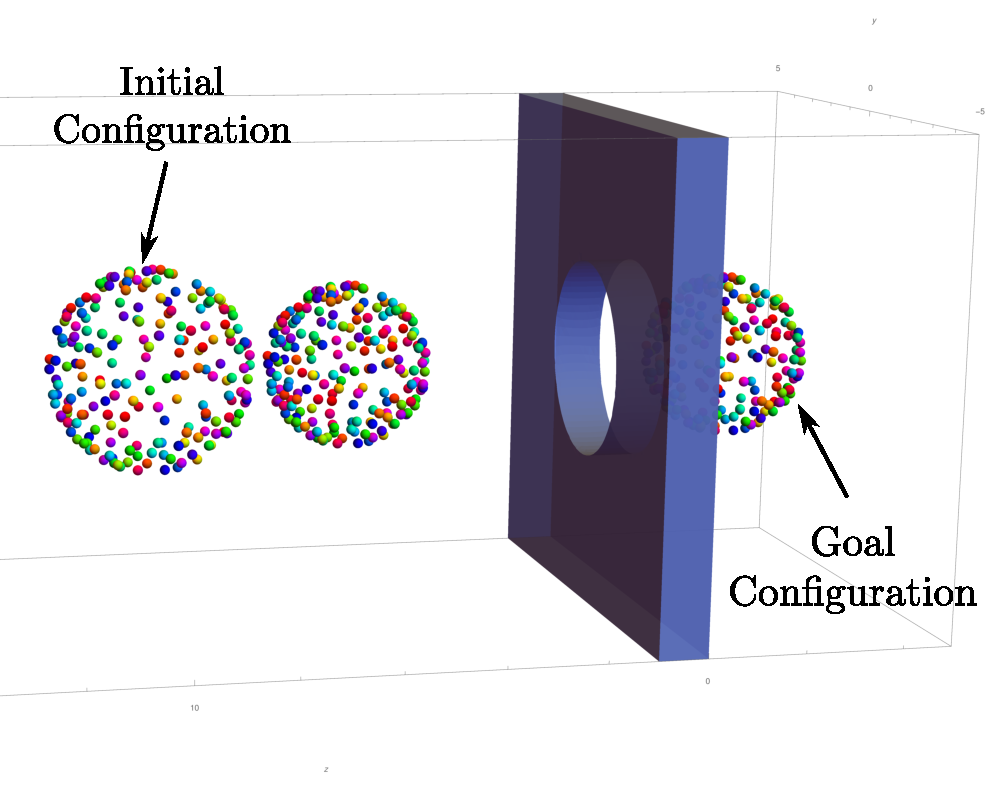
\includegraphics[width=0.5\textwidth]{r200_all}
  \caption{An example of a scenario where robots need to change their scale in order to
  pass through a narrow openning. We need to ensure that the scale parameter is computed
  such that the robots do not collide with
themselves.}
  \label{fig:r200}
\end{figure}

\subsection{Problem Description}
Consider a team of $n$ robots. These robots are arranged in a desired shape given by $\mv S =(\vsj^\top), j = 1, \ldots n$ with respect to a local coordinate system attached to the system of robots. The configuration of the system of robots is given by a five dimensional vector $\mv q = (x, y, z, \alpha, \theta)^\top$, where $\mv q_t = (x, y, z)^\top$ defines the location in the $\mathbb R^3$ space, $\alpha$ is the scale parameter for the robots, and $\theta$ is the orientation of the formation about the $Z$-axis. The location of the individual robots in the world coordinate system can now be written as $\mv p_j = \mv q_t + \mv R \alpha \vsj$, where $\mv R$ is the rotation matrix corresponding to a rotation by an angle $\theta$ about the $Z$-axis. Given an initial and goal configuration, the task is then to compute an obstacle-free path in the environment.

We assume the following:
\begin{enumerate}
  \item The robots are holonomic, i.e., they can move in any direction.
  \item The position of the individual robots, and thereby the position and orientation of the robotic system can be obtained exactly.
  \item The environment in 2D or 3D is static and known, i.e., the location of the obstacles are provided exactly.
  \item There is no error in the motion of the robots, i.e., the robots move exactly as commanded.
\end{enumerate}

\subsection{Probabilistic Roadmap}
We use Probabilistic Roadmap (PRM)~\cite{kavrakiSLO96} for creating a {\em roadmap} in the configuration space of the robot. 
The roadmap here refers to an undirected graph in the configuration space where in the nodes represent configurations and the edges represent collision-free paths which the system of robots can take. 
The weight of the edges represent the cost of travelling through the two nodes of the edge. 

The PRM 

\bibliographystyle{IEEEtran}
\bibliography{bibNmacro/agarwal_MP}

\end{document}
